\documentclass{article}
\usepackage
{graphicx} % Required for inserting images
\usepackage[utf8]{inputenc}
\usepackage{hyperref}
\usepackage[letterpaper, portrait, margin=1in]{geometry}
\usepackage{enumitem}
\usepackage{amsmath}
\usepackage{booktabs}
\usepackage{graphicx}
\usepackage{float}
\usepackage{hyperref}
\usepackage[flushleft]{threeparttable}
\usepackage{textcomp}
\hypersetup
{
colorlinks=true,
    linkcolor=black,
    filecolor=black,      
    urlcolor=blue,
    citecolor=black,
}




\usepackage{titlesec}
  
\title{Homework 9 Submission}
\author{David Wilson \\ Economics 7103}

  
\begin{document}
  
\maketitle

\section{Hourly data - Stata}

\begin{enumerate}

\item Figure 1 contains the annual recycling rates in NYC compared to the control states.    
\begin{figure}[H]
    \centering
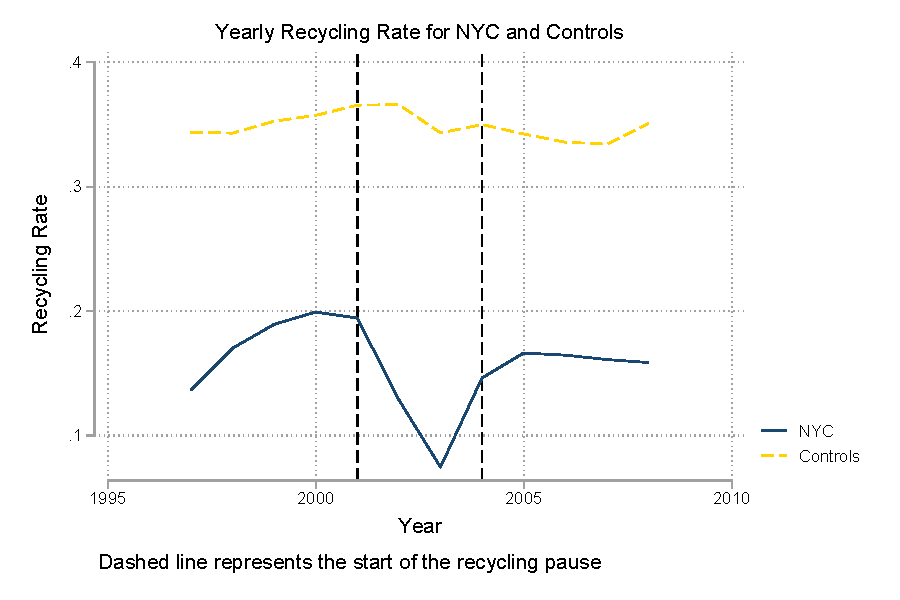
\includegraphics[width=0.6\textwidth]{HW9/nycrecyclingrate.pdf}{}
    \caption{Plot of the annual recycling rate in NYC compared to control states.}
    \label{fig:enter-label}
\end{figure}

\item The coefficient is -0.0619874 with a standard error of 0.0058221.

\item The average treatment effect for SDID is -0.06436 with a standard error of 0.00664. 

\begin{figure}[H]
    \centering
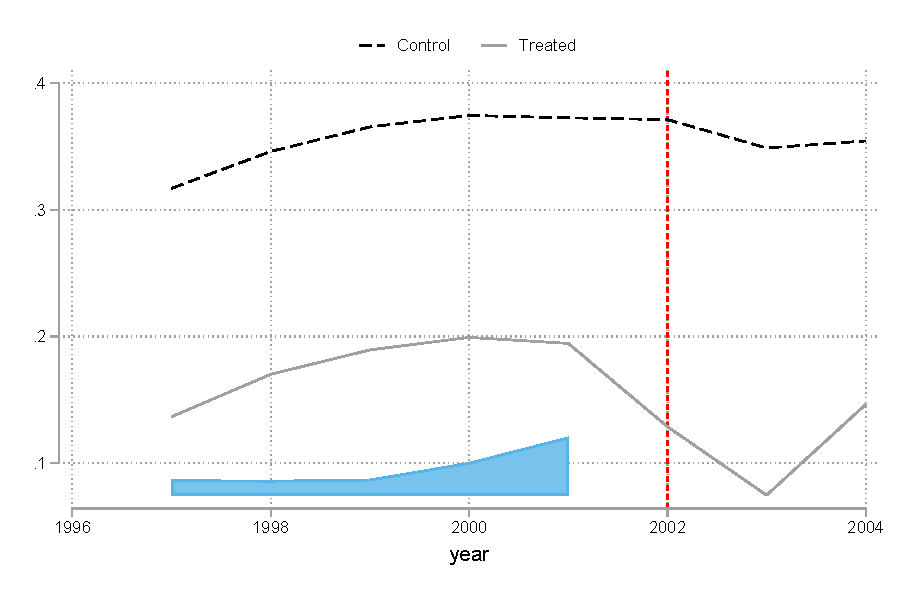
\includegraphics[width=0.6\textwidth]{HW9/sdid.pdf}{}
    \caption{Event study plot of the $\beta_l$.}
    \label{fig:enter-label}
\end{figure}

\item Event study regression using coefplot.

\begin{figure}[H]
    \centering
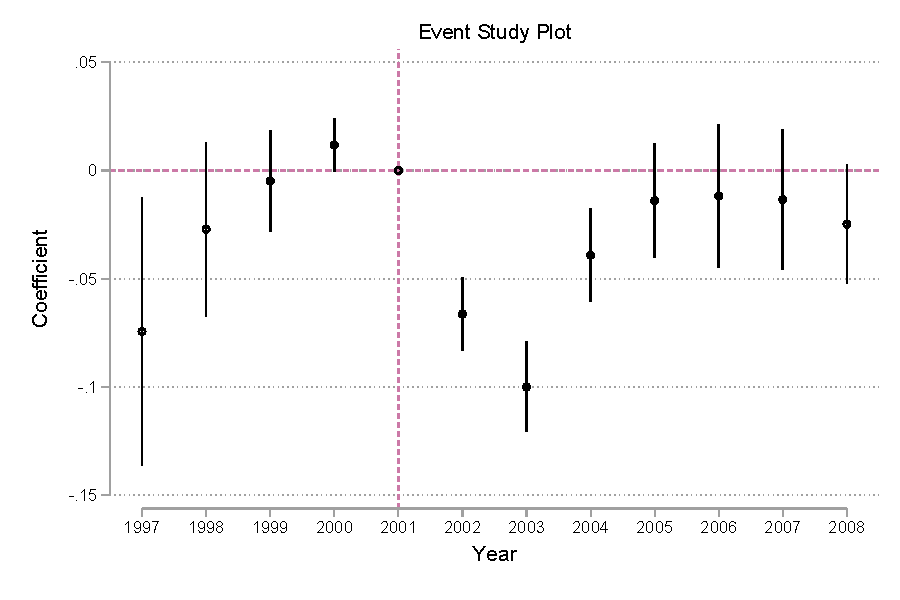
\includegraphics[width=0.6\textwidth]{HW9/eventstudyreg.pdf}{}
    \caption{Event study plot of the $\beta_l$.}
    \label{fig:enter-label}
\end{figure}

\item Reports of synthetic control estimates:           

\begin{figure}[H]
    \centering
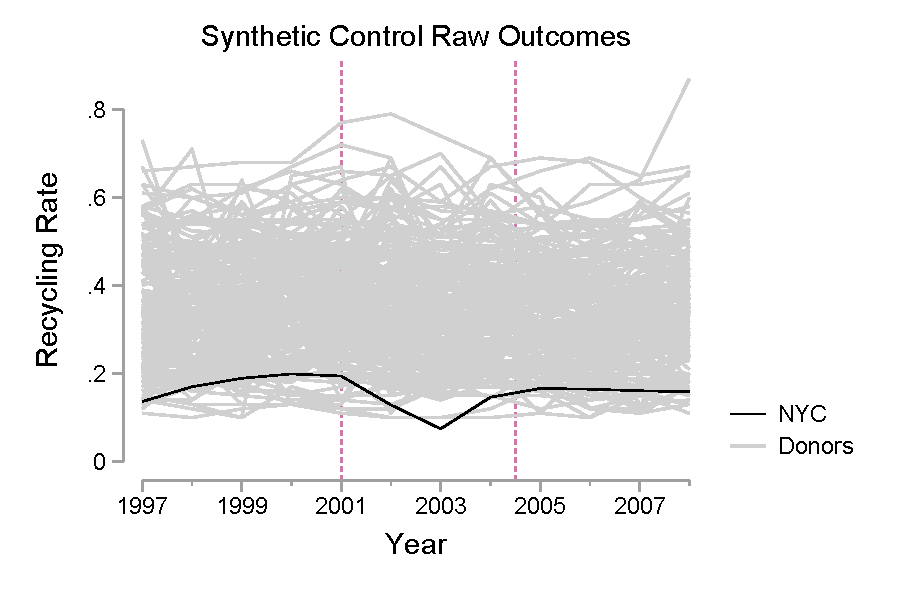
\includegraphics[width=0.6\textwidth]{HW9/raw_outcomes.pdf}{}
    \caption{The plot of raw outcomes for treated and control groups over time.}
    \label{fig:enter-label}
\end{figure}

\begin{figure}[H]
    \centering
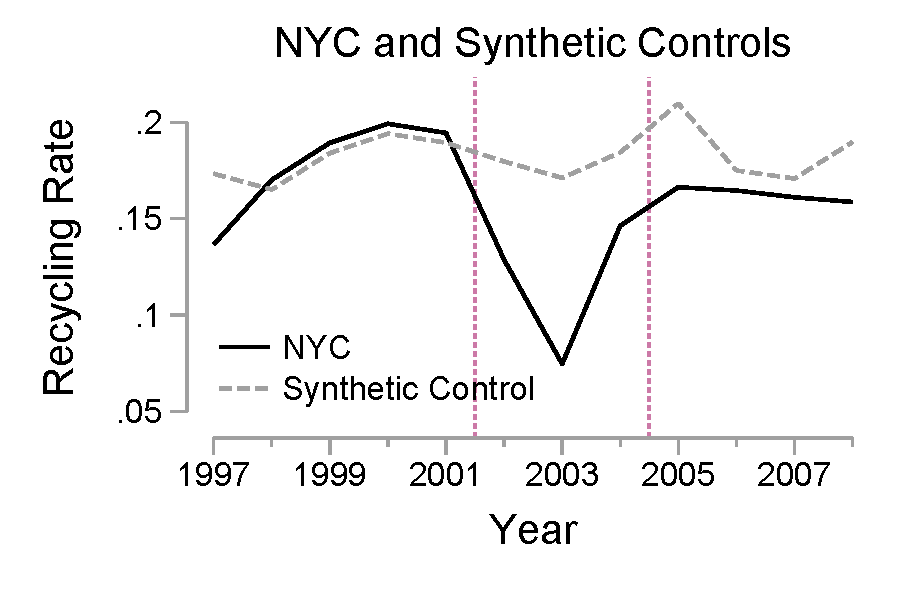
\includegraphics[width=0.6\textwidth]{HW9/treatmentcontrol.pdf}{}
    \caption{The plot of raw outcomes for treated group and synthetic control group over time.}
    \label{fig:enter-label}
\end{figure}

\begin{figure}[H]
    \centering
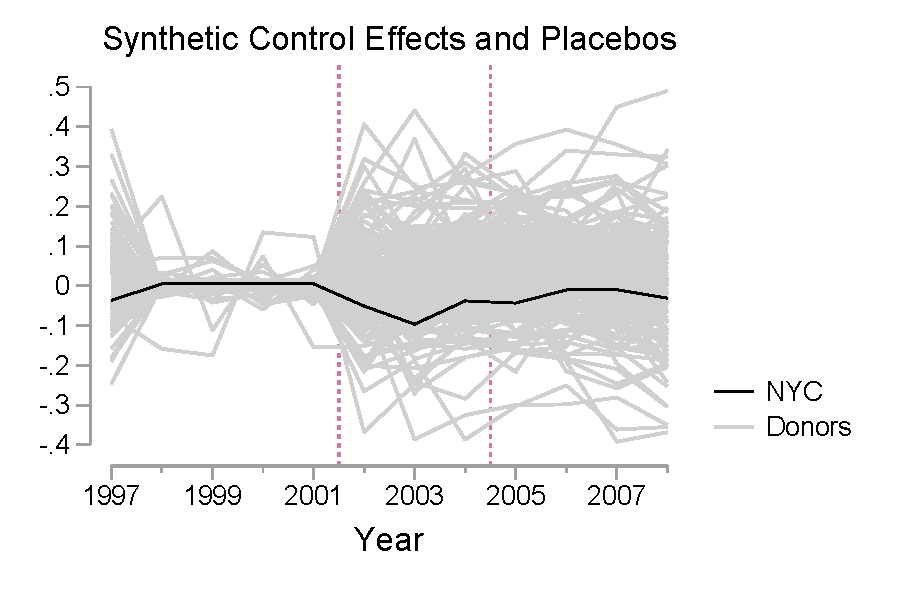
\includegraphics[width=0.6\textwidth]{HW9/placeboeffects.pdf}{}
    \caption{The plot of estimated synthetic control effects and placebo effects over time.}
    \label{fig:enter-label}
\end{figure}

\begin{figure}[H]
    \centering
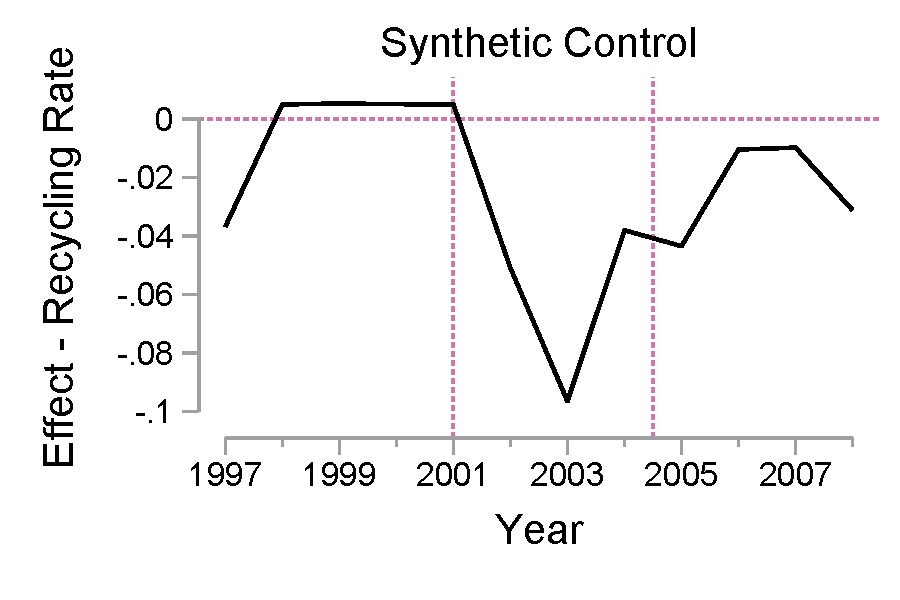
\includegraphics[width=0.6\textwidth]{HW9/effect.pdf}{}
    \caption{The plot of final synthetic control estimates over time.}
    \label{fig:enter-label}
\end{figure}
\end{enumerate} 
   
 \end{document}

